\chapter{大图可视化的相关工作}\label{chap:大图可视化的相关工作}

本章内容首先叙述了数据规模对可视化方法的影响,主要集中在布局和交互两个方面。第\ref{A-sec:数据规模对可视化方案的影响}、\ref{A-sec:大规模图布局技术的发展}小节从布局计算的角度回顾了图布局算法的发展;第\ref{图数据抽样算法}小节补充了目前针对大图数据在交互上的方法和优化策略。

\section{图布局算法的发展}\label{A-sec:数据规模对可视化方案的影响}

... deleted ...


    \subsection{单核串行阶段}

    ... deleted ...

    \begin{table}[h]
        \centering
        \bicaption{可视化分析工具比较。}{Comparison of visualization tools}
        \fontsize{10}{10}\selectfont
        \setlength{\tabcolsep}{0.7mm}{
        \begin{tabular}{lllcclcl}
            \toprule
            名称 & 出现 & 最新版本 & 免费 & 开源 & 语言 & 动态布局 & 主要功能 \\
            \midrule
            Ucinet & 1992 & 2011.11 & × & × & Delphi & × & 分析 \\
            Pajek & 1996 & 2019.3 & √ & × & Delphi & √ &  分析、可视\\
            NetMiner & 2001 & 2019.2 & × & × & Java & × &  分析、可视\\
            NodeXL & 2008 & 2019.4 & × & √ & C\# & √ &  可视、分析、交互\\
            Gephi & 2009 & 2017.9 & √ & √ & Java & √ &  可视、分析、交互\\
            Visone & 1996  & 2017.2 & √ & ×  & Java  & ×  &  可视、分析 \\
            Graphviz & 2000  & 2019.2 & √ & √  & dot  & × & 可视、分析、交互  \\
            Network Workbench & 2005  & 2011.3 & √ & ×  &  C++ & ×  & 可视、分析  \\
            SocNetV & 2014  & 2019.3 & √ & √  & C++/Qt  & ×  &  分析、可视、交互 \\
            Tulip &  2000 & 2019.4  & √ & √  & C++  & √  & 分析、可视、交互  \\

            \bottomrule
        \end{tabular}%
        }
    \end{table}\label{tab:tools}


    ... deleted ...

    之后,Kamada和Kawai\citep{kamada1989algorithm}对其做了改进,引入了非邻居节点间最佳距离的概念(最佳距离\emph{l}同非邻两节点间的最短路径成正比),并首次将整个布局过程抽象为能量降低(最优化)的问题,通过最小化节点间斥力和引力的和,来将节点放置在合理的位置,整个系统中的能量模型可用公式\ref{forum:Eades-Layout}表示,

    \begin{equation}\label{forum:Eades-Layout}
    Eenergy = \sum\limits_{0 \le {\rm{i < j}} \le {\rm{|V|}}} {{k_{ij}}} {(|{x_i} - {x_j}| - {l_{ij}})^2}
    \end{equation}

    其中$x_{i}$为顶点$v_{i}$对应的坐标位置,$k_{ij}$为$x_{i}$与$x_{j}$之间连接弹簧的弹力系数,$l_{ij}$为顶点$v_{i}$与$v_{j}$之间的最佳距离。该方法每次只求取一个点的最佳位置,即其内循环(单次算法执行)时间复杂度为$O(|V|)$。


    ... deleted ...


    \subsection{单机并行阶段}\label{A-sec:单机并行阶段}

    ... deleted ...

\section{大规模图布局技术的基础}\label{A-sec:大规模图布局技术的发展}

... deleted ...


    \subsection{分布式存储计算平台}

    \begin{enumerate}
        \item ... deleted ...
        \item ... deleted ...
        \begin{itemize}
            \item ... deleted ...
            \item ... deleted ...
            \item ... deleted ...
            \item ... deleted ...
        \end{itemize}

    \end{enumerate}

    \subsection{大规模图数据处理框架}

    ... deleted ...

    \begin{figure}[!htbp]
        \centering
        %trim option's parameter order: left bottom right top
        % \includegraphics[trim = 30mm 0mm 30mm 0mm, clip, width=0.40\textwidth]{shock_cyn}
        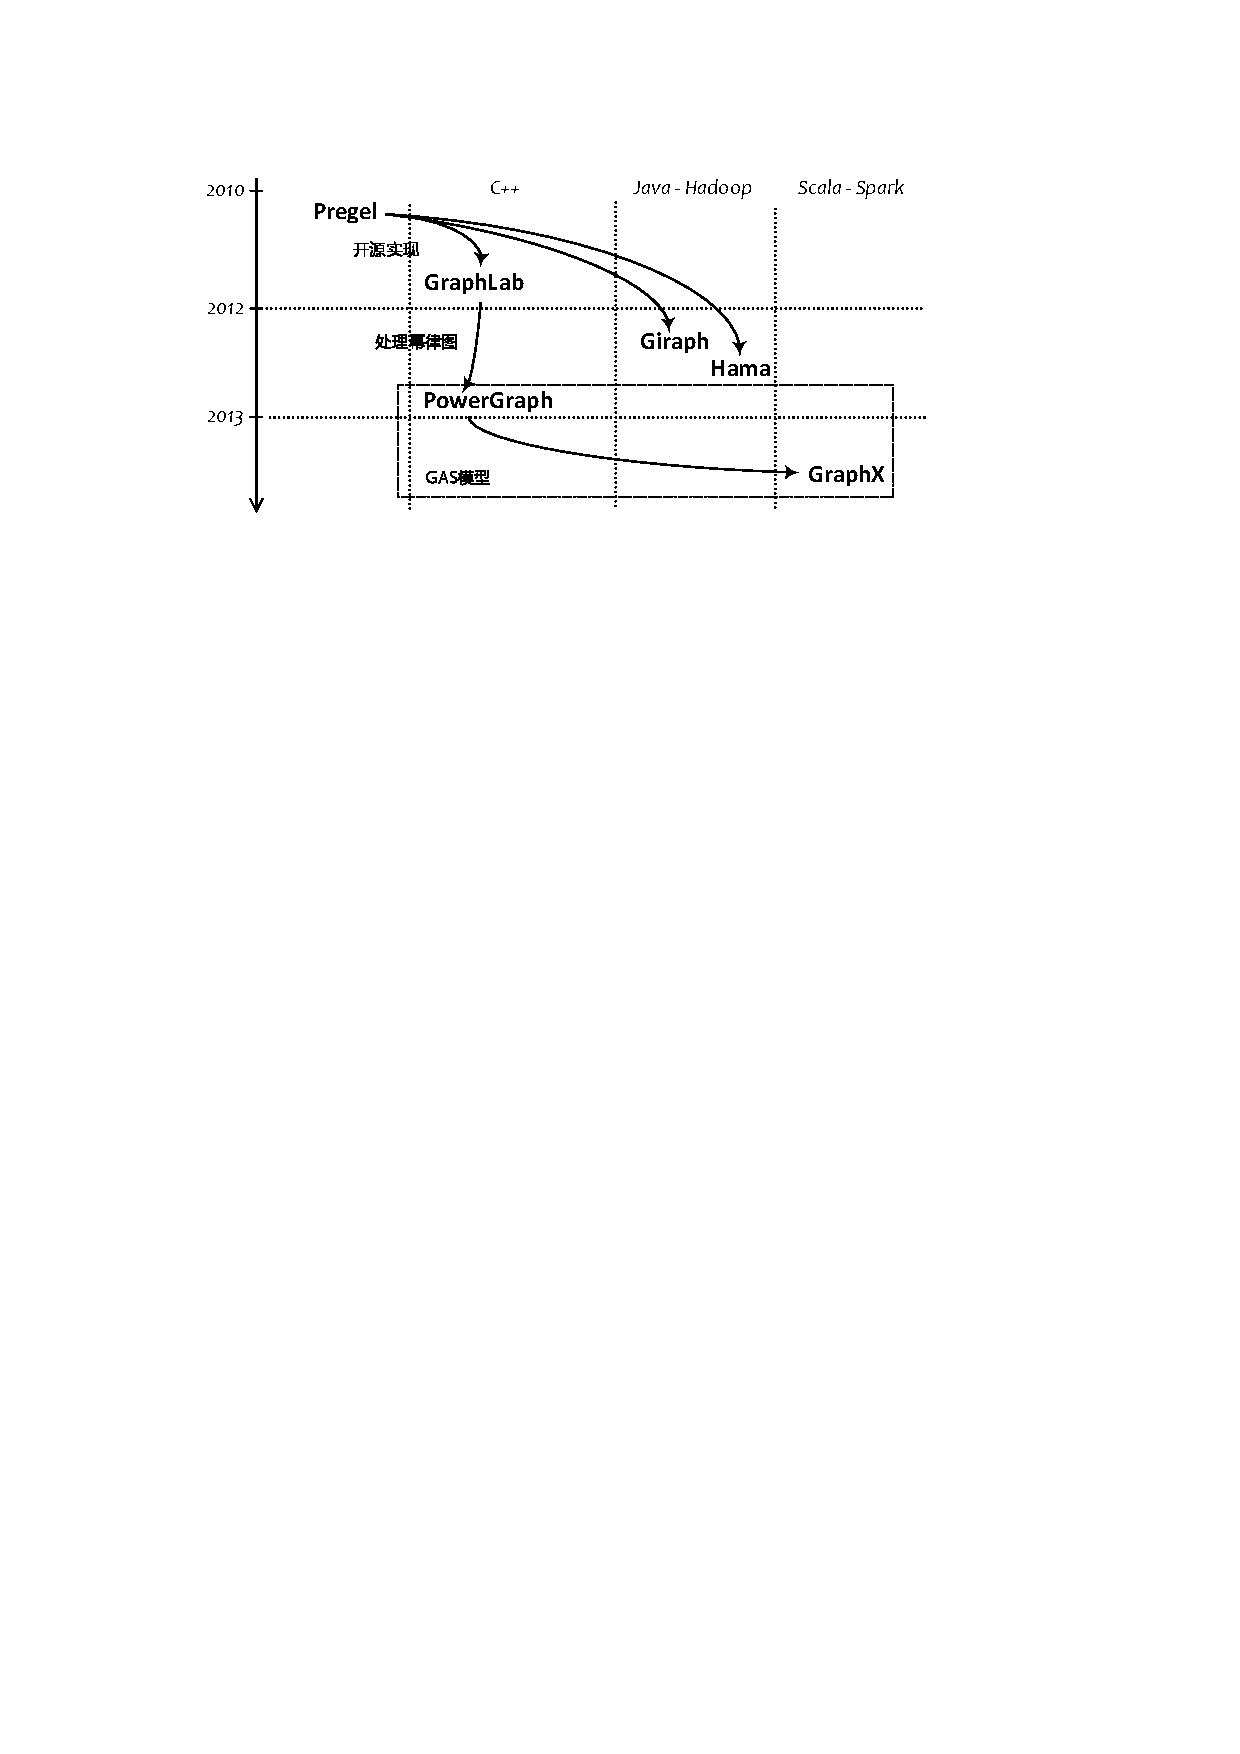
\includegraphics[width=0.80\textwidth]{vis-3-bsp}
        \bicaption{(分布式)图计算框架的发展历程。}{Development of (distributed) graph computing framework.}
        \label{fig:vis-3-bsp}
    \end{figure}

    \begin{enumerate}

        \item ... deleted ...
        \item ... deleted ...
        \item ... deleted ...
            \begin{itemize}
            \item ... deleted ...
            \item ... deleted ...
            \item ... deleted ...
            \end{itemize}

        \item ... deleted ...

            \begin{figure}[!htbp]
                \centering
                %trim option's parameter order: left bottom right top
                % \includegraphics[trim = 30mm 0mm 30mm 0mm, clip, width=0.40\textwidth]{shock_cyn}
                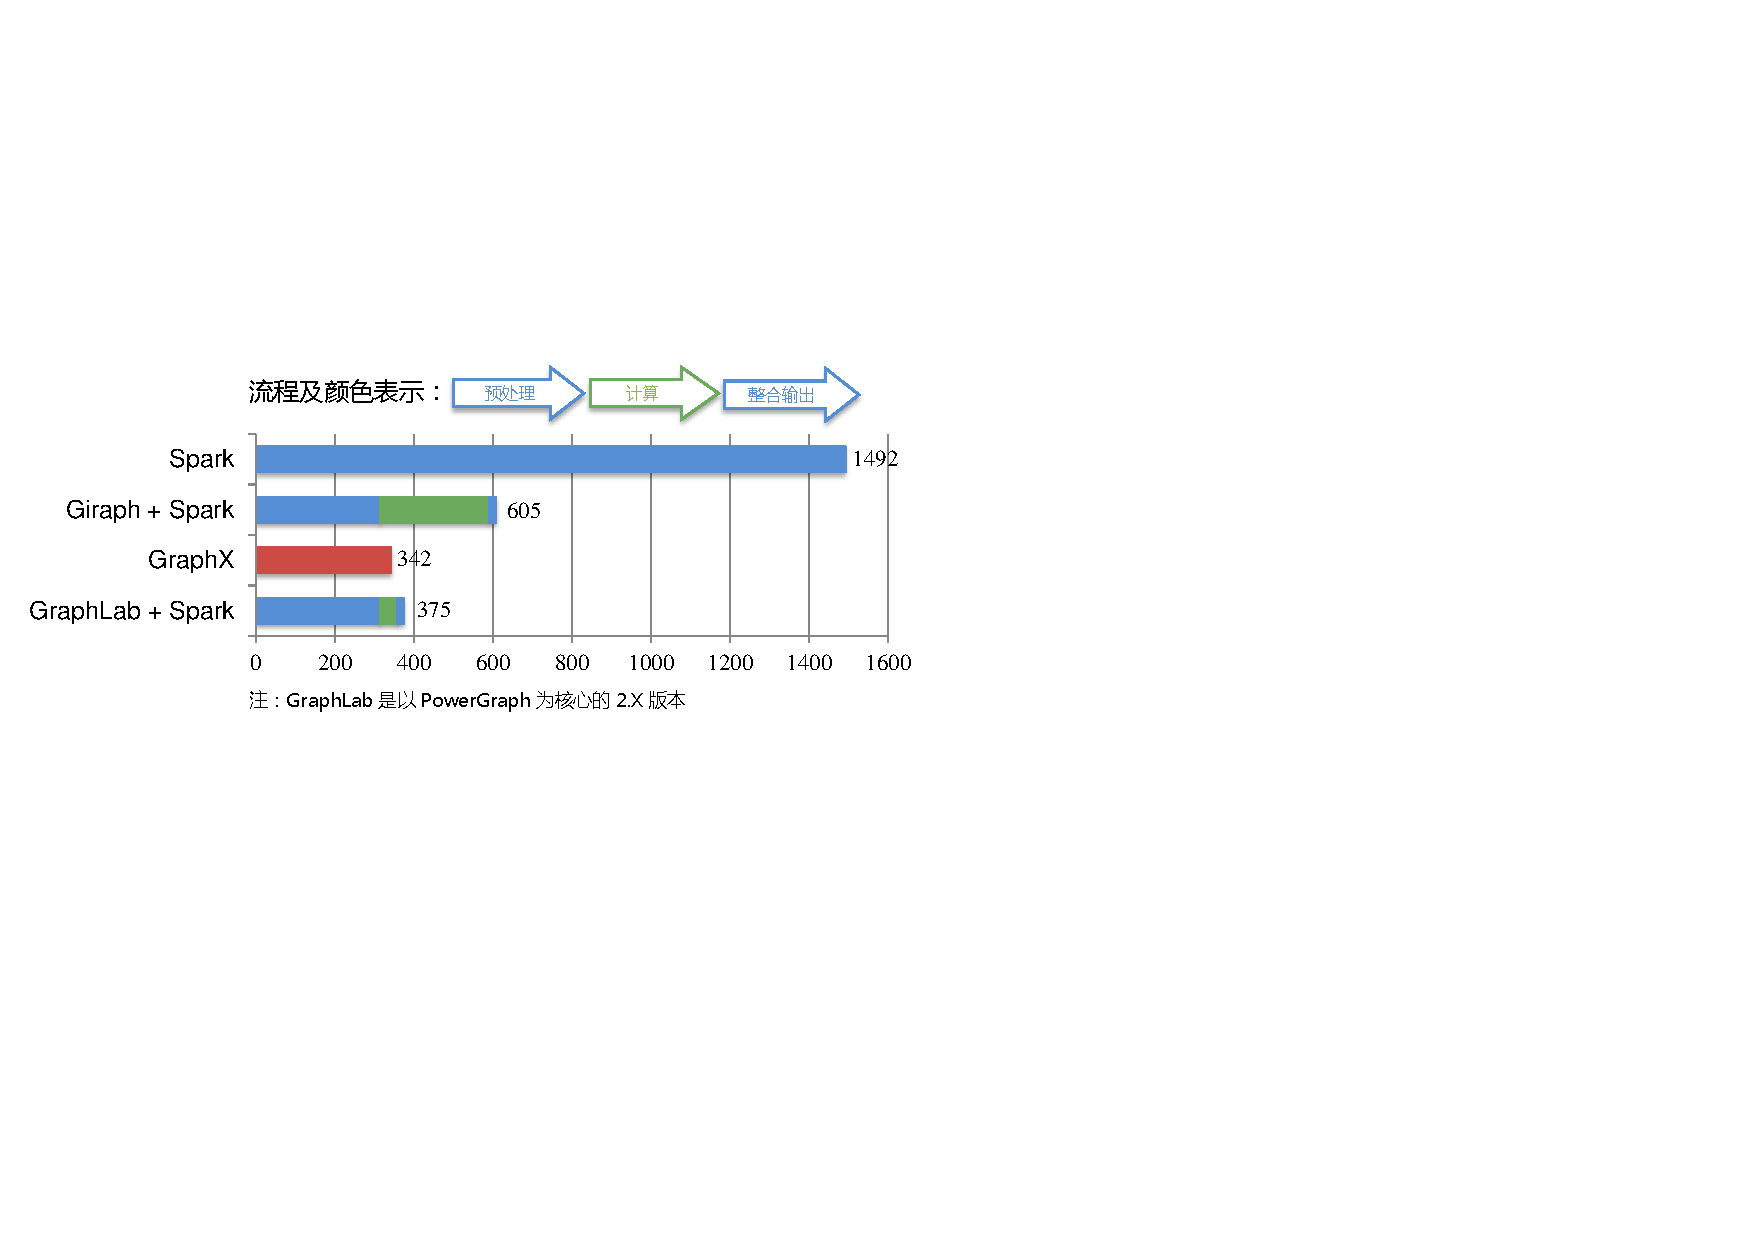
\includegraphics[width=0.85\textwidth]{vis-3-graphxplus}
                \bicaption{Pipeline模式下的性能分析-10次PageRank的运行时间。}{Performance test based on pipeline mode - Times of 10 PageRank iterations.}
                \label{fig:vis-3-graphxplus}
            \end{figure}

 
    \end{enumerate}

    \subsection{大规模图布局算法}

    ... deleted ...
 
    \section{图数据抽样算法}\label{图数据抽样算法}

    ... deleted ...





\section{本章小结}

... deleted ...